%----------------------------------------------------------------------------------------
% Biobank V4 Design
%
% The latest version of this document is kept on GitHub at:
%
% https://github.com/cbsrbiobank/biobankv4design
%
%----------------------------------------------------------------------------------------

\documentclass[10pt,twoside,letterpaper]{memoir}
% Page margins
\usepackage[top=3cm,bottom=3cm,left=3.2cm,right=3.2cm,headsep=10pt,a4paper]{geometry}

\usepackage[T1]{fontenc}
\usepackage{titlesec} % Allows customization of titles

\usepackage[english]{babel} % English language/hyphenation
\usepackage{booktabs} % Required for nicer horizontal rules in tables
\usepackage{graphicx} % Required for including pictures

\usepackage[svgnames]{xcolor} % Required to specify font colors

\usepackage{bookman} % font used for text
\usepackage{csquotes}

\usepackage{microtype} % Slightly tweak font spacing for aesthetics
\usepackage[utf8]{inputenc} % Required for including letters with accents
\usepackage{enumitem} % allows lists to be customized

\DeclareMathAlphabet{\mathpzc}{OT1}{pzc}{m}{it}
\DeclareGraphicsExtensions{.pdf,.png,.jpg}

%----------------------------------------------------------------------------------------
% Colors used in document
%----------------------------------------------------------------------------------------

\definecolor{Blue}{rgb}{.204,.353,.541}
\definecolor{LightBlue}{RGB}{76,129,188}
\definecolor{Green}{RGB}{155,186,87}
\definecolor{Orange}{RGB}{248,150,71}
\definecolor{Purple}{RGB}{129,99,162}
\definecolor{gray75}{gray}{0.75}

%----------------------------------------------------------------------------------------
% PDF settings
%----------------------------------------------------------------------------------------

\usepackage[pdftex,
  pdfauthor={AICML},
  pdftitle={BioBank V4 Design},
  colorlinks,
  linkcolor=Blue,
  bookmarks=true,
  bookmarksopen=true,
  pdfstartview=FitH]
	   {hyperref}

\hypersetup{
  citecolor=Blue,
  linkcolor=Purple
}

%----------------------------------------------------------------------------------------
% Bibliography settings
%----------------------------------------------------------------------------------------

\usepackage[
  style=alphabetic,
  sorting=nyt,
  sortcites=true,
  autopunct=true,
  babel=hyphen,
  hyperref=true,
  abbreviate=false,
  backref=true,
  backend=biber
]{biblatex}
\addbibresource{bibliography.bib} % BibTeX bibliography file
\defbibheading{bibempty}{}

%----------------------------------------------------------------------------------------
% Chapter and section formating - using 'ell' chapter style with customizations
%----------------------------------------------------------------------------------------

\chapterstyle{ell}
\renewcommand*{\chapnumfont}{\normalfont\Huge\bfseries\sffamily\color{Blue}}
\renewcommand*{\chaptitlefont}{\normalfont\Huge\bfseries\sffamily\color{Blue}}
\renewcommand*{\secheadstyle}{\normalfont\Large\bfseries\sffamily\color{Blue}}
\renewcommand*{\subsecheadstyle}{\normalfont\Large\bfseries\sffamily\color{LightBlue}}

\setcounter{secnumdepth}{3}
\setsecnumdepth{subsection}

%----------------------------------------------------------------------------------------
%	TITLE PAGE
%----------------------------------------------------------------------------------------

\newcommand*{\titleTH}{\begingroup % Create the command for including the title page in the document
\raggedleft % Right-align all text
\vspace*{\baselineskip} % Whitespace at the top of the page

% Author % name
{\Large\bfseries\sffamily Author: Nelson Loyola}\\[0.167\textheight]

{\hfill\rule{.7\textwidth}{2pt}}\vspace*{\baselineskip}

% First part of the title
{\LARGE\bfseries\sffamily Biobank V4}\\[\baselineskip]

% Main title which draws the focus of the reader
{\textcolor{Blue}{\Huge\bfseries\sffamily Design Document}}\\[\baselineskip]

{\large\bfseries\sffamily \textit{Draft 0.1}}

{\hfill\rule{.7\textwidth}{2pt}}

% Whitespace between the title block and the publisher
\vfill

% Publisher and logo
{\large\bfseries\sffamily
  \href{http://biosample.ca/}{Prepared for the Canadian Biosample Repository} \\
  by the \href{http://www.aicml.ca/}{Alberta Innovates Center for Mathine Learning}\\ }\par
\vspace*{\baselineskip}
{\textcolor{Blue}{
    \small\sffamily University of Alberta\\
    Department of Computing Science\\
    2-21 Athabasca Hall\\
    Edmonton, Alberta\\
    \href{mailto:info@aicml.ca}{info@aicml.ca}
}}

\vspace*{3\baselineskip} % Whitespace at the bottom of the page
\endgroup}

%----------------------------------------------------------------------------------------
% Ttable of contents
%----------------------------------------------------------------------------------------

\usepackage[textsize=small, backgroundcolor=Orange, bordercolor=Orange, shadow]{todonotes}

\renewcommand{\cftchapterfont}{\normalfont\bfseries\sffamily}
\renewcommand{\cftsectionfont}{\normalfont\sffamily}
\renewcommand{\cftsubsectionfont}{\normalfont\sffamily}
\renewcommand{\cftchapterpagefont}{\normalfont\sffamily\bfseries}
\renewcommand{\cftsectionpagefont}{\normalfont\sffamily}
\renewcommand{\cftsubsectionpagefont}{\normalfont\sffamily}

\maxtocdepth{subsection}

\AtBeginDocument{\renewcommand\contentsname{Table of Contents}}

%----------------------------------------------------------------------------------------
% document macros
%----------------------------------------------------------------------------------------

\newcommand{\entitytarget}[1]{\hypertarget{#1}{#1}}
\newcommand{\valobjtarget}[1]{\hypertarget{#1}{#1}}

\newcommand{\entitylink}[1]{\hyperlink{#1}{\texttt{\textbf{#1}}}}
\newcommand{\valobjlink}[1]{\hyperlink{#1}{\texttt{\textbf{#1}}}}


%----------------------------------------------------------------------------------------
% Document start
%----------------------------------------------------------------------------------------

\begin{document}
\frontmatter

\thispagestyle{empty} % Removes page numbers
\titleTH % This command includes the title page

\clearpage
\tableofcontents
\clearpage
%\listoffigures
%\clearpage
%\listoftodos
%\clearpage

\mainmatter
\chapter{Introduction}

Biobank version 4 is a rewrite of the Biobank application, meant to provide the
majority of its functionality through a web browser based interface. It was
designed using Domain Driven Design principles \cite{evans2004domain} and
employs a CQRS architecture (Command Query Responsibility Segregation)
\cite{vernon2013implementing}.

In addition, version 4 includes enhancements to the domain model which provides
better workflow and an improved user experience.

Flatbed scanning is supported by having a separate dedicated client, but this
client's functionality is focused only on scanning and decoding tubes etched
with 2D barcodes.

\section{Dependencies}

This version of Biobank uses the following open source tools / software packages:

% table with no indentation
\begin{description}

  \item[Jetty Http Server] \hfill \\ The Embedded Jetty Server provides web
    browser with access to the application.

  \item[MongoDB ] \hfill \\ A document based NoSQL database and provides an
    event store implementation that stores event streams in a MongoDB database.

  \item[MySQL database ] \hfill \\ A SQL relational database management sytem
    used to store the query model.

  \item[Axon Framework ] \hfill \\ Provides the building blocks used in
    applying the CQRS architectural pattern.

  \item[Spring Framework ] \hfill \\ Provides a comprehensive programming and
    configuration model for modern Java-based enterprise applications.

  \item[Spring MVC ] \hfill \\ Model-view-controller framework for web
    applications.

  \item[Spring Security ] \hfill \\ A customizable authentication and
    access-control framework for securing web applications.

  \item[Hibernate ] \hfill \\ An object-relational mapping library that
    provides a framework to map a data model to a relational database.

  \item[Twitter Bootstrap ] \hfill \\ Bootstrap is a sleek, intuitive, and
    powerful front-end framework for faster and easier web user interface
    development \cite{bootstrap}

\end{description}

\section{CQRS}

There are a number of reasons for choosing the CQRS architecture for
Biobank. Amongst these are:

\begin{itemize}
\item Employs a message-based system that allows for decoupling and is more
  reliable against transient failures.
\item \textbf{Commands} (that change data) are separated from \textbf{queries}
  (that read data).
\item Enables domain driven design by capturing the intent in the form of
commands.
\item \textbf{Event Sourcing} allows persisting of application entities as a
  sequence of events that created them. Thus, captures all business changes in a
  lossless manner.
\item Events are used to populate views also known as the reporting side. Thus,
  allows for decoupling of domain logic from reporting.
\item Allows for definitions of new reports that provide new insight to the
  data that has already been captured.
\end{itemize}

\chapter{Architecture}

\section{External Architecture}

The Biobank application uses a hexagonal architecture to interface to internal
and external clients, external services, and for data storage. Figure
\ref{fig:hex-architecture} shows the how the ports are configured. Web browser
based clients access the application via the internal client port. A RESTful
interface is also supported to allow the Biobank scanning client access via the
external client port. External systems can also access the application via this
port. Biobank can communicate to external services by using the external
services port. The figure also shows that the event store and query databases
are accessed via dedicated ports.

\begin{figure}[h]
  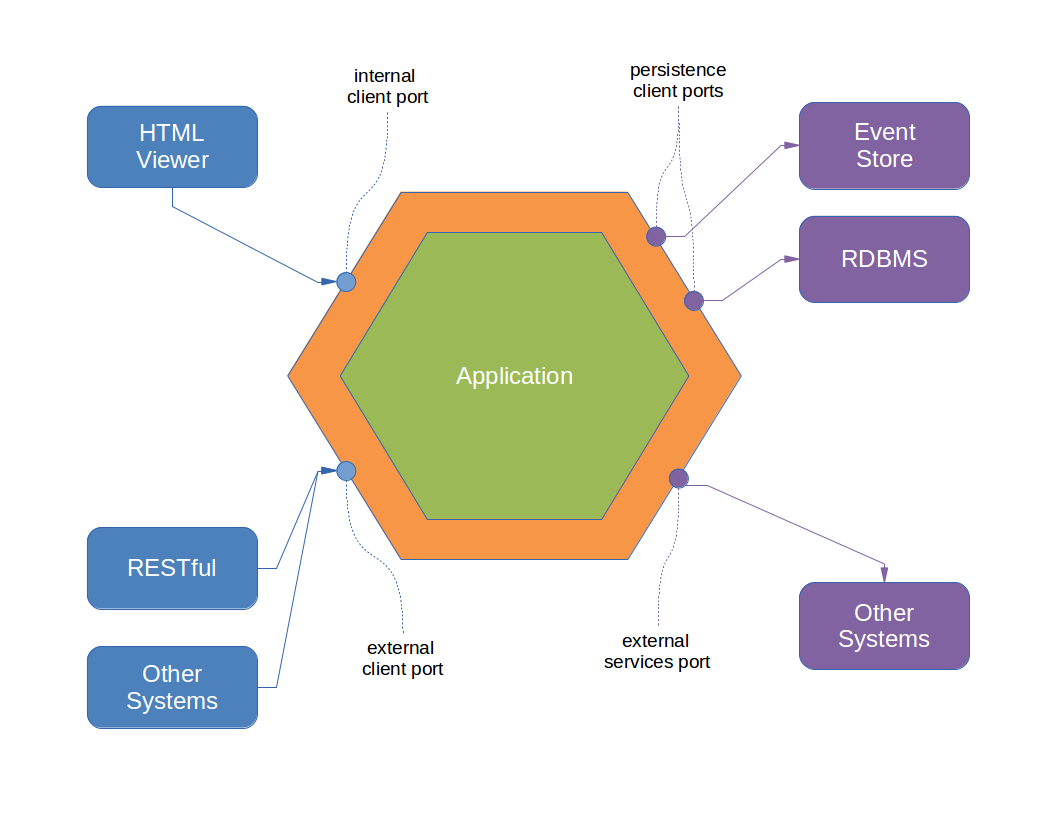
\includegraphics[trim={15mm 18mm 15mm 12mm}, clip, width=1\textwidth]{images/hex-architecture}
  \caption{Hexagonal architecture}
  \label{fig:hex-architecture}
\end{figure}

\section{Interal Architecture}

The client ports shown in Figure \ref{fig:hex-architecture} are managed by
client adapters. These client adapters then interface to the rest of the system
via the \emph{Command Bus} and the \emph{Query Interface} provided by the
\emph{Thin Data Layer}. Figure \ref{fig:cqrs-architecture} shows a more detailed
view of the application. It is the architecture recommended by the Axon
Framework\footnote{The figure and the material that follows is borrowed from
  the Axon Framework Reference Guide \cite{AxonOnline}}.

\begin{figure}[h]
  \begin{center}
    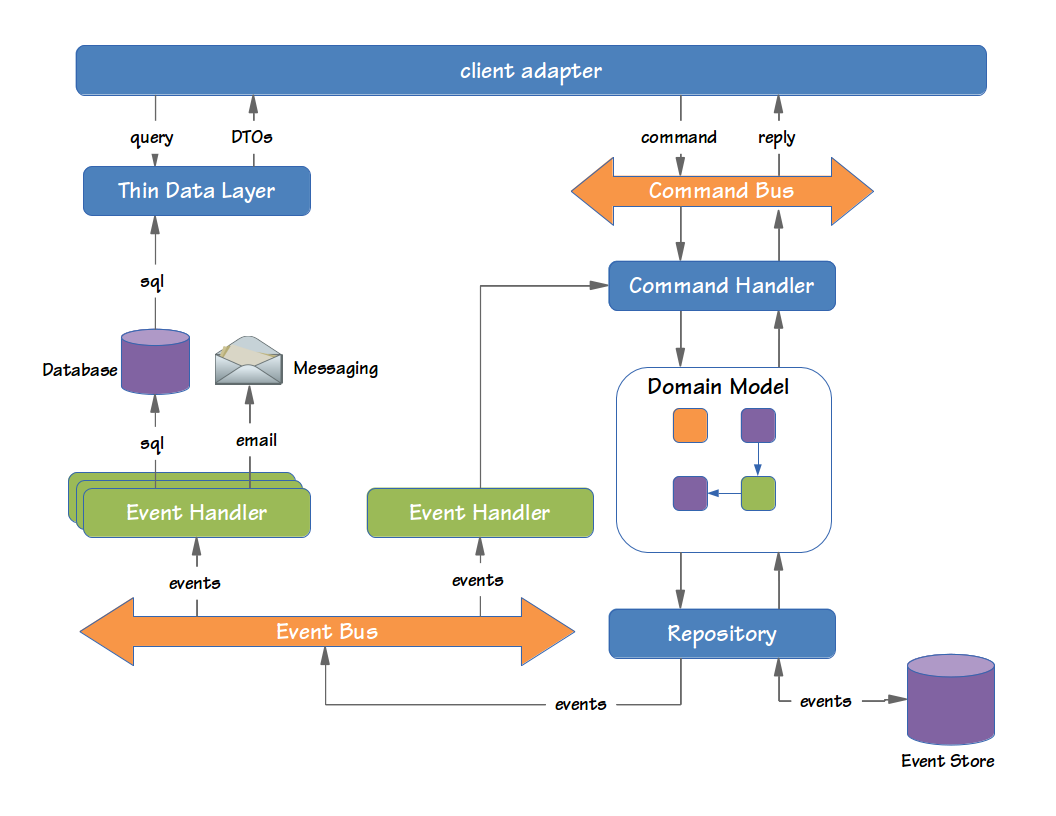
\includegraphics[trim={10mm 5mm 15mm 10mm}, clip, width=1\textwidth]{images/cqrs-architecture}
    \caption{Biobank architecture}
    \label{fig:cqrs-architecture}
  \end{center}
\end{figure}

\section*{Command Handling}

Commands are typically represented by simple and straightforward objects that
contain all data necessary for a command handler to execute it. A command
expresses its intent by its name. In Java terms, that means the class name is
used to figure out what needs to be done, and the fields of the command provide
the information required to do it.

The Command Bus receives commands and routes them to the Command Handlers. Each
command handler responds to a specific type of command and executes logic based
on the contents of the command. In some cases, however, logic is executed
regardless of the actual type of command, such as validation, logging or
authorization.

\section*{Domain Model}

The command handler retrieves domain objects (Aggregates) from a repository and
executes methods on them to change their state. These aggregates typically
contain the actual business logic and are responsible for guarding their own
invariants. The state changes of aggregates result in the generation of Domain
Events. Both the Domain Events and the Aggregates form the domain model.

\section*{Repositories and Event Stores}

Repositories are responsible for providing access to aggregates. Typically,
these repositories are optimized for lookup of an aggregate by its unique
identity. Repositories store the state changes that the aggregate has gone
through in an Event Store. The repository is also responsible for persisting
the changes made to aggregates in its backing storage.

\section*{Event Processing}

The event bus dispatches events to all interested event handlers. This is done
synchronously or asynchronously. Asynchronous event dispatching allows the
command execution to return and hand over control to the user, while the events
are being dispatched and processed in the background. Not having to wait for
event processing to complete makes an application more responsive. Synchronous
event processing, on the other hand, is simpler and is a sensible
default. Synchronous processing also allows several event listeners to process
events within the same transaction.

Event handlers receive events from the event bus. Some handlers update data
sources used for querying while others send messages to external
systems. Command handlers are completely unaware of the components that are
interested in the changes they make. This means that it is very non-intrusive
to extend the application with new functionality. All you need to do is add
another event handler. The events loosely couple all components in your
application together.

In some cases, event processing requires new commands to be sent to the
application. The saga is the CQRS concept responsible for managing these
complex business transactions.

\section*{Querying for data}

The thin data layer in between the client adapters and the data sources
provides a clearly defined interface to the actual query implementation
used. This data layer typically returns read-only Data Transfer Objects (DTOs)
containing query results. The contents of these DTOs are typically driven by
the needs of the client adapters. In most cases, they map directly to a
specific view in the UI (also referred to as table-per-view).

\subsection{Axon Framework Modules}

The Axon Framework provides a number of different modules that target specific
problem areas of CQRS. This section describes which modules were chosen.

\todo[inline]{This section is incomplete.}

\chapter{Domain Model}

The Biobank application is composed different modules\footnote{The term ``Module''
  is used in the context described in \cite{vernon2013implementing}}. Each
module is described briefly here and in more details are provided in the
remaining chapters.


\begin{description}

  \item[Study Configuration] \hfill \\

  \item[Patient Collection] \hfill \\

  \item[Specimen Processing] \hfill \\

  \item[Center Shipment] \hfill \\

  \item[Center Configuration] \hfill \\

  \item[Center Storage Configuration] \hfill \\

  \item[Specimen Request] \hfill \\

\end{description}

\chapter{Study Management}

\section{Entities}

The entities in this module are:

\begin{description}

  \item[Study] \hfill \\
    Represents a collection of participants and specimens collected for a
    particular research study. The study is part of an aggregate that define
    the types of specimens to be collected and how they are to be collected
    from participants.

  \item[] \hfill \\

  \item[] \hfill \\

  \item[] \hfill \\

  \item[] \hfill \\

  \item[] \hfill \\

  \item[] \hfill \\


\end{description}

\section{Value Objects}

The value objects in this module are:

\begin{description}

  \item[Study] \hfill \\

  \item[] \hfill \\

  \item[] \hfill \\

  \item[] \hfill \\

  \item[] \hfill \\

  \item[] \hfill \\

  \item[] \hfill \\


\end{description}


%----------------------------------------------------------------------------------------
% Bibliography
%----------------------------------------------------------------------------------------

\chapter*{Bibliography}
\addcontentsline{toc}{chapter}{Bibliography}
\printbibliography[heading=bibempty]

\end{document}
